% \documentclass[conference,10pt]{ieeeconf}
\documentclass[letterpaper, 10 pt, conference]{ieeeconf}
\IEEEoverridecommandlockouts
\overrideIEEEmargins
\usepackage{pstricks}
\usepackage{ifplatform}
\usepackage{xkeyval}
\usepackage{rotating}
\newtheorem{remark}{Remark}
\usepackage{graphics} % for pdf, bitmapped graphics files
% TEST-DEL: \usepackage[off]{auto-pst-pdf}
% \usepackage{mathptmx} % assumes new font selection scheme installed
\usepackage{times} % assumes new font selection scheme installed
\usepackage{amsmath} % assumes amsmath package installed
\usepackage{psfrag}
\usepackage{cancel}
\def\etal{\mbox{et al.}}
% \usepackage{pifont}
% \usepackage{flushend}
\usepackage[normalem]{ulem}
\usepackage{cite}
\usepackage{url}
\usepackage{color}
\input rgb
\def\blue#1{\textcolor{blue}{#1}}
\def\red#1{\textcolor{red}{#1}}
\def\orange#1{\textcolor{orange}{#1}}
\def\green#1{\textcolor{darkgreen}{#1}}
\usepackage{comment}
\usepackage{amssymb}
\usepackage{amsfonts}
%\usepackage[caption=false,font=footnotesize]{subfig}
\usepackage{subcaption}
% \usepackage{mathptmx}
%\usepackage{enumitem}
\usepackage{algorithmic}
\usepackage{algorithm}
\usepackage{pifont}% http://ctan.org/pkg/pifont
\newcommand{\cmark}{\ding{51}}%
\newcommand{\xmark}{\ding{55}}%
\newcommand{\smark}{$\bigstar$}%
\usepackage{booktabs}
%\input lamacro
\usepackage{lipsum}
\usepackage{array}
\newcolumntype{P}[1]{>{\centering\arraybackslash}p{#1}}
\newcommand{\JT}[1]{\textcolor{blue}{JT: #1}}
\newcommand{\AC}[1]{\textcolor{green}{AC: #1}}
\newcommand{\LP}[1]{\textcolor{red}{}}
\newcommand{\MN}[1]{\textcolor{orange}{MN: #1}}

\newcommand{\GR}[1]{\textcolor{magenta}{GR: #1}}
\newcommand{\assigned}[1]{\textcolor{purple}{Assigned To: #1}}
\newcommand{\budget}[1]{\textcolor{purple}{Page Budget: #1}}

\newcommand{\longonly}[1]{}
\newcommand{\shortonly}[1]{#1}

\newcommand{\maybeRemove}[1]{{\color{gray}#1}}
\newcommand{\xxx}{\textbf{\color{red}???}}
\newcommand{\LPafter}[1]{\longonly{\LP{#1}}}

% \renewcommand{\LP}[1]{}



\let\clipbox\relax
\usepackage{adjustbox}
%\usepackage{array}
\usepackage{booktabs}

\usepackage{CJKutf8}

\newcolumntype{R}[2]{%
    >{\adjustbox{angle=#1,lap=\width-(#2)}\bgroup}%
    l%
    <{\egroup}%
}
\newcommand*\rot{\multicolumn{1}{R{70}{1em}}}

\graphicspath{{figures/},{figures/new_diagrams/}}
\newcommand{\svgpath}{./images}

\usepackage{hyperref}
%\let\oldsection\section
%\renewcommand{\section}{\clearpage\oldsection}

%\allowdisplaybreaks[2]
\renewcommand{\baselinestretch}{0.97}
\textfloatsep = 6pt

% \let\subparagraph\relax
% \usepackage{titlesec}
% \usepackage[compact]{titlesec}
% \titlespacing{\section}{0pt}{2ex}{1ex}
% \titlespacing{\subsection}{0pt}{1ex}{0ex}
% \titlespacing{\subsubsection}{0pt}{0.5ex}{0ex}

\usepackage{mdwlist}
\let\stditemize\itemize
\let\endstditemize\enditemize
\let\itemize\undefined
\makecompactlist{itemize}{stditemize}

\let\stdenumerate\enumerate
\let\endstdenumerate\endenumerate
\let\enumerate\undefined
\makecompactlist{enumerate}{stdenumerate}

\setlength{\abovecaptionskip}{1pt}
\setlength{\belowcaptionskip}{1pt}

\usepackage[tracking=false,kerning=true,spacing=true]{microtype}
\pdfprotrudechars=2
\pdfadjustspacing=2

\title{\LARGE \bf
Duckieboat: 小型水上無人載具設計、開發與應用}

\author{Jui-Te Huang$^{1}$, Shao-Huang Lu$^{2}$, and Tzu-Kuan Chuang$^{1}$}

\begin{document}
%\begin{CJK}{UTF8}{bsmi}
\begin{CJK}{UTF8}{bkai}

    \maketitle

    \thispagestyle{empty}
    \pagestyle{empty}

    %%%%%%%%%%%%%%%%%%%%%%%%%%%%%%%%%%%%%%%%%%%%%%%%%%%%%%%%%%%%%%%%%%%%%%%%%%%%%%%%

    \begin{abstract}

Duckieboat is an Unmanned maritime vehicle. Due to the cost of building an unmanned maritime vehicle is very expensive and time consuming. We decide to design a low-cost, high-durability, modular-design and easy-assemble boat which can implement in our research. It is also capable of transform into a variety of water applications, such as boat following, material supply, garbage collection and difficult environment marine exploration. We hope our Duckieboat will enhance the safety of sea in the future and can make the supply of water sports enthusiasts more convenient. Duckieboat also can implement in the teaching field, make students learn more about the related principles of autonomous boat.

Keywords: Unmanned System, Autonomous Navigation, Marine Robotics

\end{abstract}


    %%%%%%%%%%%%%%%%%%%%%%%%%%%%%%%%%%%%%%%%%%%%%%%%%%%%%%%%%%%%%%%%%%%%%%%%%%%%%%%%
    \section{Introduction}

Duckieboat is an Unmanned maritime vehicle. Due to the cost of building an unmanned maritime vehicle is very expensive and time consuming. We decide to design a low-cost, high-durability, modular-design and easy-assemble boat which can implement in our research. It is also capable of transform into a variety of water applications, such as boat following, material supply, garbage collection and difficult environment marine exploration. We hope our Duckieboat will enhance the safety of sea in the future and can make the supply of water sports enthusiasts more convenient. Duckieboat also can implement in the teaching field, make students learn more about the related principles of autonomous boat.

    \section{Hardware Structure}

\begin{figure}[h] % h means put this image here
	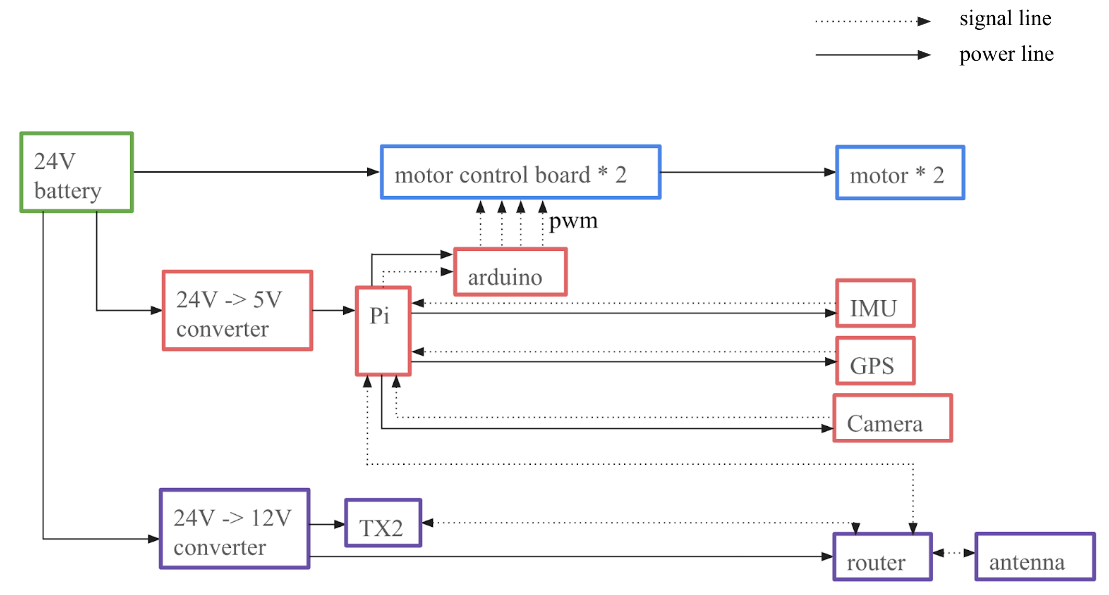
\includegraphics[width=0.8\columnwidth]{images/hardware.png}
	\centering
	\caption{signal and power flow}
	\label{figure:hardware}
\end{figure}

\subsection{Power Transmition}

For power transmission, this system needs 3 kinds of voltages, 24V, 5V, and 12V. 24V supply through two motor control boards then drive the two motors. 5V supply initially powered Raspberry pi, it will also supply Arduino UNO, IMU, GPS and pi camera with it’s USB ports. As to 12V, it will supply TX2 compute unit and router.

\subsection{Signal Transmition}

For signal transmission, Raspberry pi and TX2 will communicate through wifi, wifi router with an antenna will set on the boat. The Raspberry pi will collect the data from IMU, GPS and pi camera, after computing in Raspberry pi and image processing in TX2, it will send pwm signal (0~3.3V) to Arduino UNO, then Arduino will map the input signal from (0~3.3V) into (0~5V) to two motor control boards.

\subsection{hardware setting}
Most of the compute units and sensors mentioned above except two motors, GPS and antenna, will be placed in a waterproof box. There will have waterproof connectors while the wire needs to go out from the waterproof box.

\begin{figure}[h] % h means put this image here
	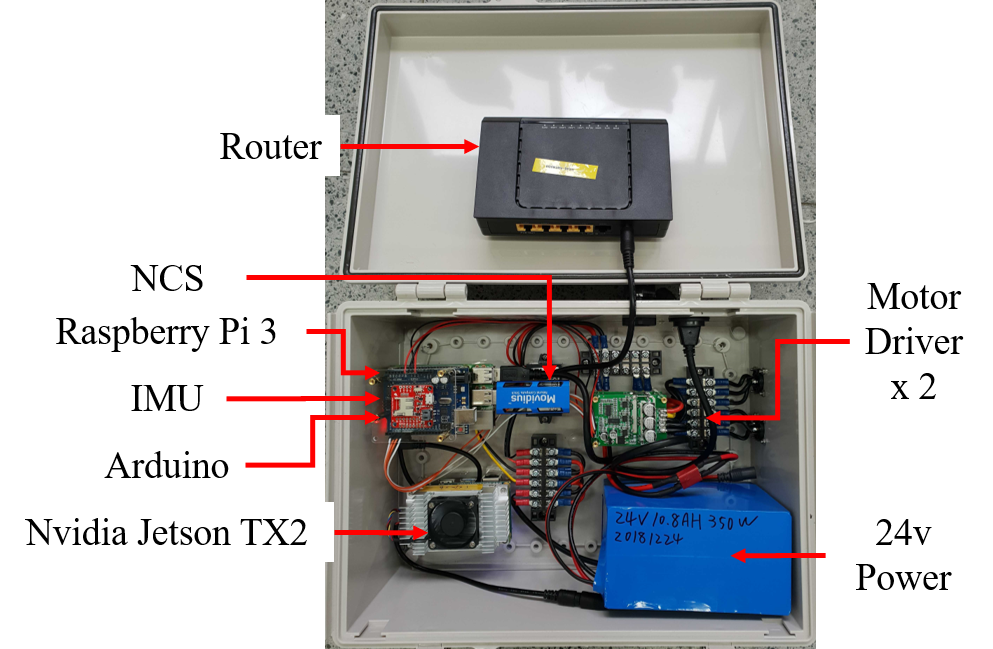
\includegraphics[width=0.8\columnwidth]{images/hardware_setting.png}
	\centering
	\caption{hardware setting}
	\label{figure:hardware_setting}
\end{figure}

\begin{figure}[h] % h means put this image here
	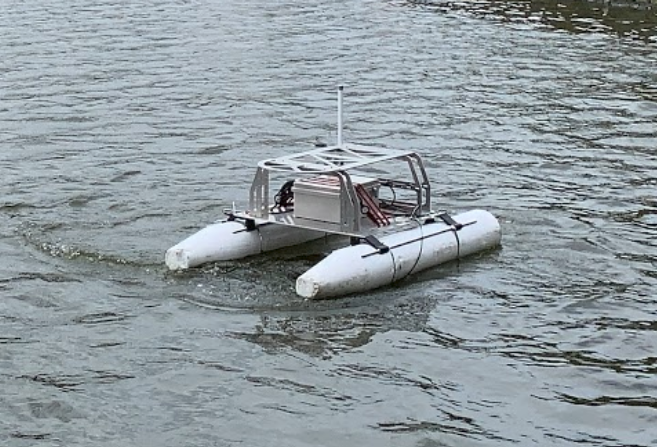
\includegraphics[width=0.8\columnwidth]{images/duckieboat.png}
	\centering
	\caption{The appearance of Duckieboat and where the waterproof box was placed.}
	\label{figure:duckieboat}
\end{figure}


    \section{Software Structure}

\subsection{Joystick Control}

We use ROS write a node to switch between autonomous motor command and user control motor command.

\subsection{Waipoint Navigation}

We use GPS and IMU data to create Odometry. And it is filtered by a kalman filter then we pass our odometry to the navigation node to creat the motor command.

\subsection{Track and Trail}

To track the object on the water surface. We use pi-camera to get the image ahead of the boat. Then pass this image to object detection node. Once detect the object. we pass the bounding box of the object to the tracking node. Finally create a motor command to the Joystick node.

\begin{figure}[h]
	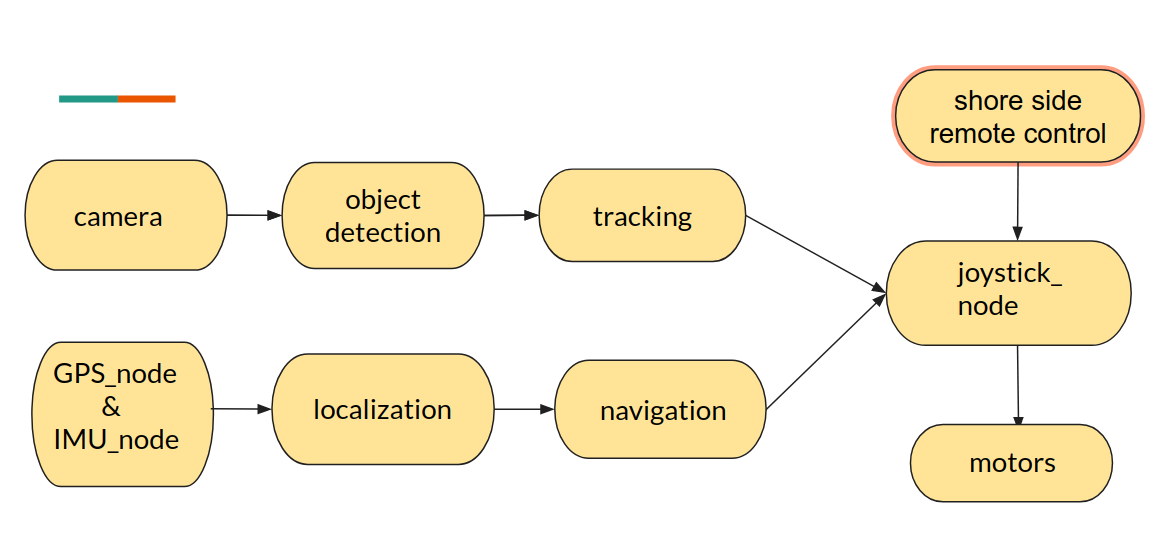
\includegraphics[width=0.8\columnwidth]{images/software_structure.png}
	\centering
	\caption{software structure}
	\label{figure:software_structure}
\end{figure}

    %\section{實驗與實體驗證}

\subsection{機器人定位與避障任務}

本研究先以微小化平台測試所建置的感測塔、系統與演算法,將於期末報告對大型無人載具(地面與水面)平台進行測試。

\paragraph{定位準確度測試}

本計畫先針對機器人定位的準確度逕行測試,測試方法比較 1) GPS與IMU進行感測融合,2) 只有GPU資料,實驗地點為交大圖書館前方空地,以一個邊長約100公尺的矩形路線,實驗人員攜帶所建置的感測塔跟著矩形路線行走,並將資料錄製於ROS Bag檔案,實驗結果如圖
\ref{table:loop_closure_error}所示。結果顯示,從出發點經過指定路線後,回到原始點的誤差值在兩組硬體設定相差不大,但於GPU+IMU設定標準差的值較小,表示在定位過程較穩定。

\begin{table}[h]
	\centering
	\begin{tabular}{| c| c| c|}
		\hline
		Sensor Set & 定位誤差  x, y (m) & 路線標準差 x, y (m) \\ \hline
		GPS + IMU & 0.65, 0.83 & 0.37, 0.42 \\ \hline
		GPS only  & 0.60, 0.83 & 0.41, 0.72 \\ \hline 
	\end{tabular}
	\caption{定位測試}
	\label{table:loop_closure_error}
\end{table} 

\paragraph{避障測試於簡化實驗環境} 

本計畫先使用微小化平台,先於室內與室外較為平坦之場域測試,測試內容(請參考圖~ \ref{figure:exp-results})與影片連結如下:

\begin{itemize}

\item
巡邏點進行純追蹤演算法(Pure Pursuit Algorithm): 
\url{https://youtu.be/DdaZkm7_bjI}

\item
避障實驗一(靜態障礙物): 
\url{https://youtu.be/ve4Mln4D1xo}

\item
避障實驗二(動態障礙物):
\url{https://youtu.be/E1anLPuXjxs}

\item
無人水上載具於虛擬環境避障任務: 
\url{https://youtu.be/DBuMrUvr7iY}

\end{itemize}

\begin{figure}[h] % h means put this image here
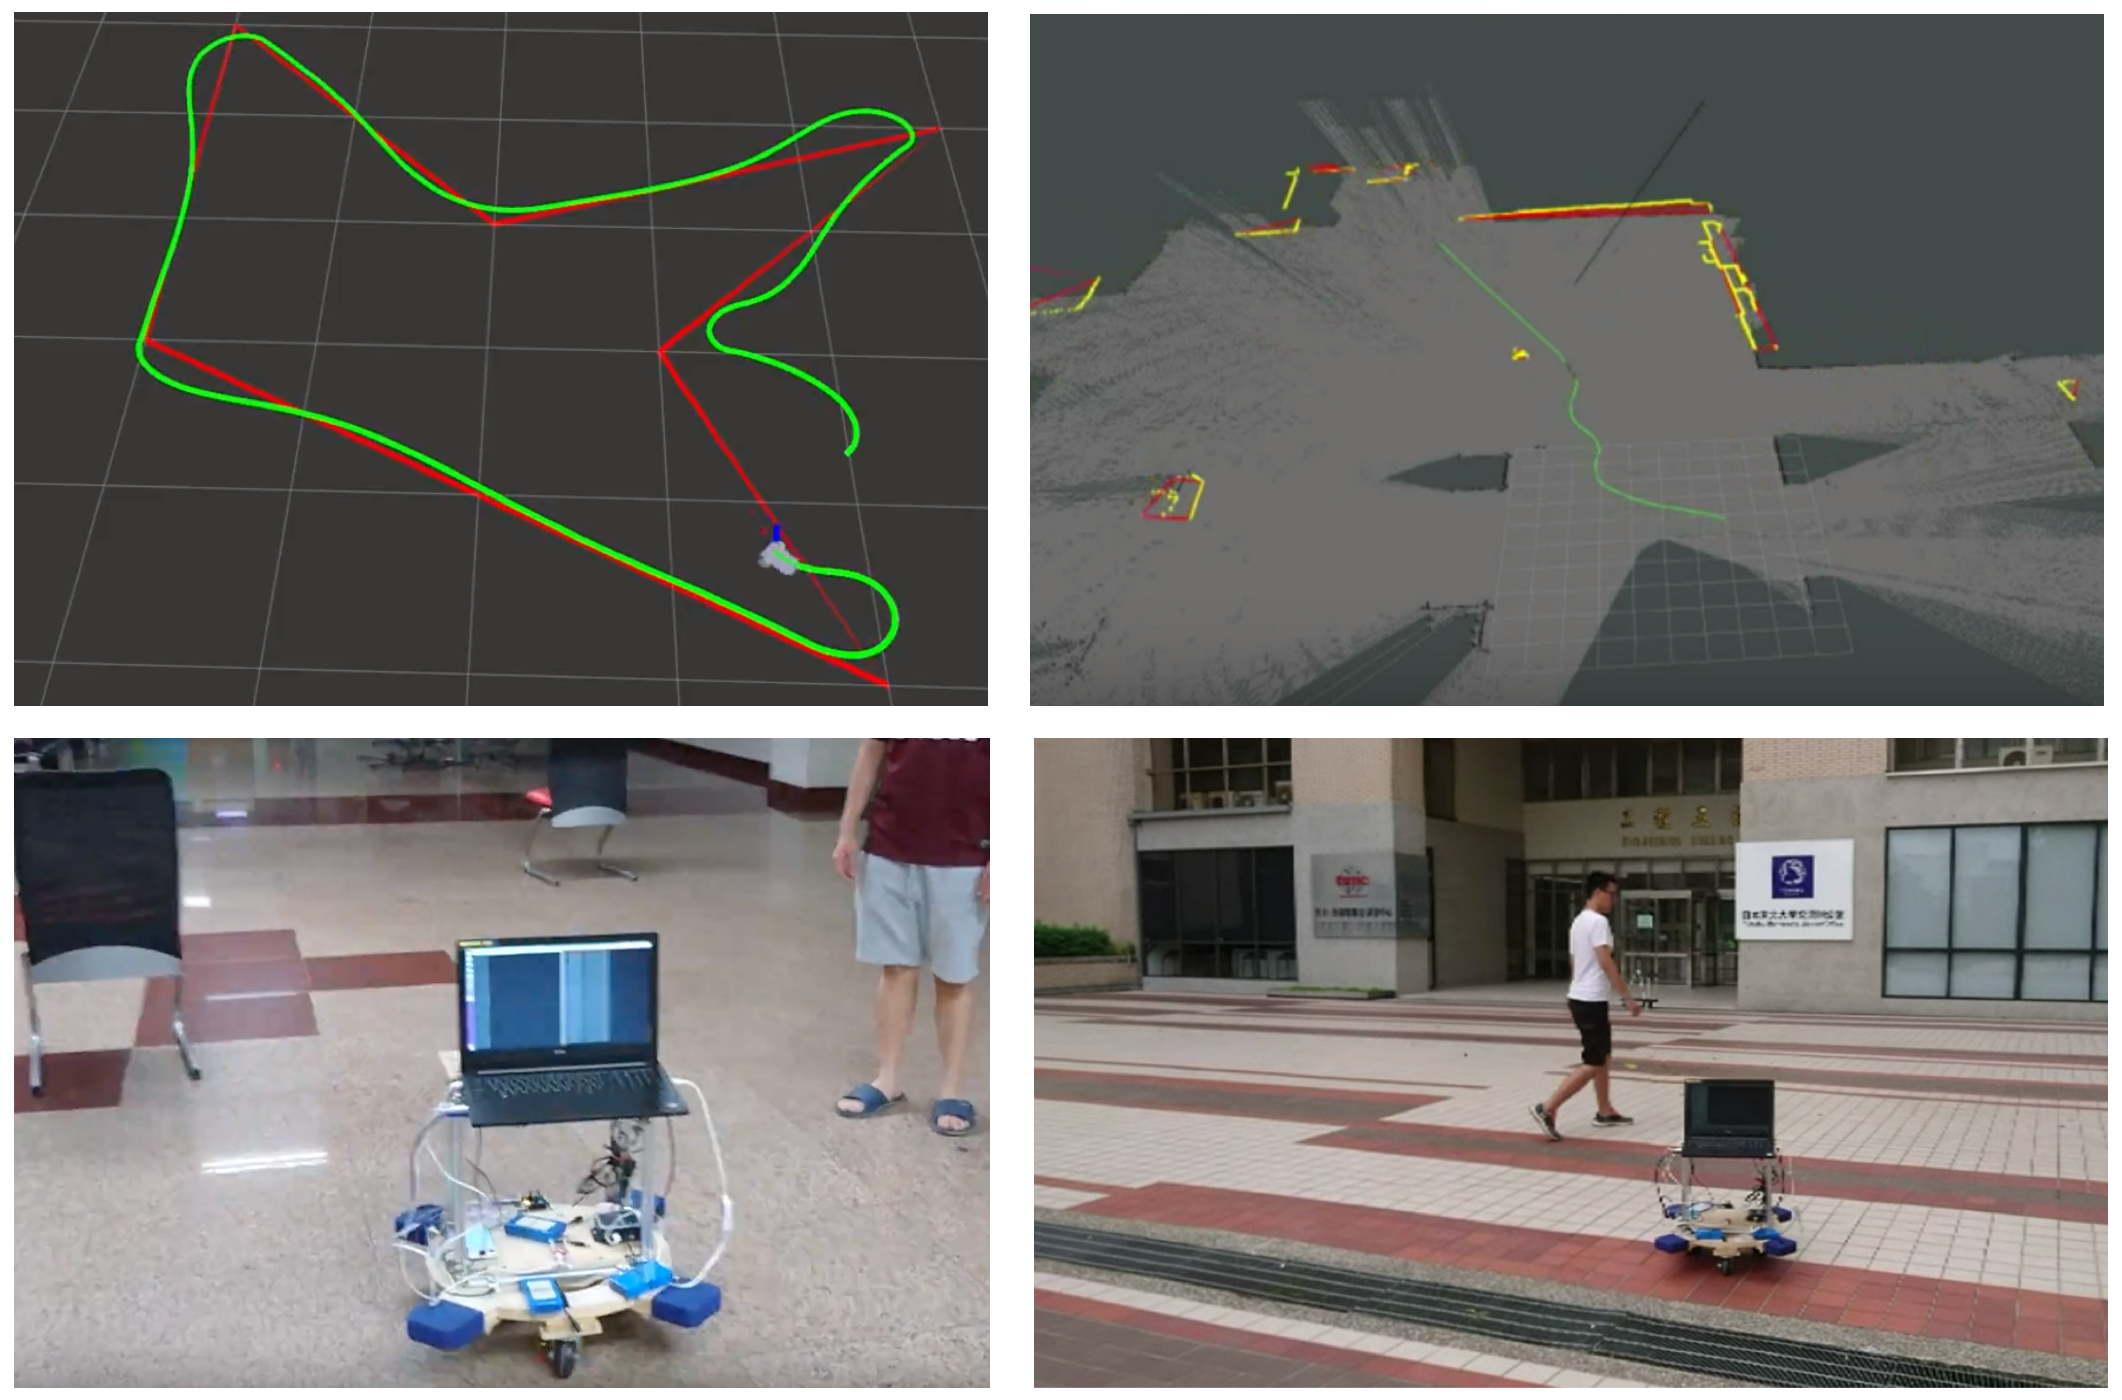
\includegraphics[width=\columnwidth]{images/exp-results.png}
\centering
\caption{微小化平台與簡化場域測試}
 \label{figure:exp-results}
\end{figure}


\subsection{地面無人載具(進行中)}

本計畫預計將所開發之演算法用於大型地面無人載具(Clearpath Husky,請參考圖~\ref{figure:ground-vehicle}),結合所開發的點雲及開發演算法於地形模擬建構,於不平坦之崎嶇地形進行測試。

\begin{figure}[h] % h means put this image here
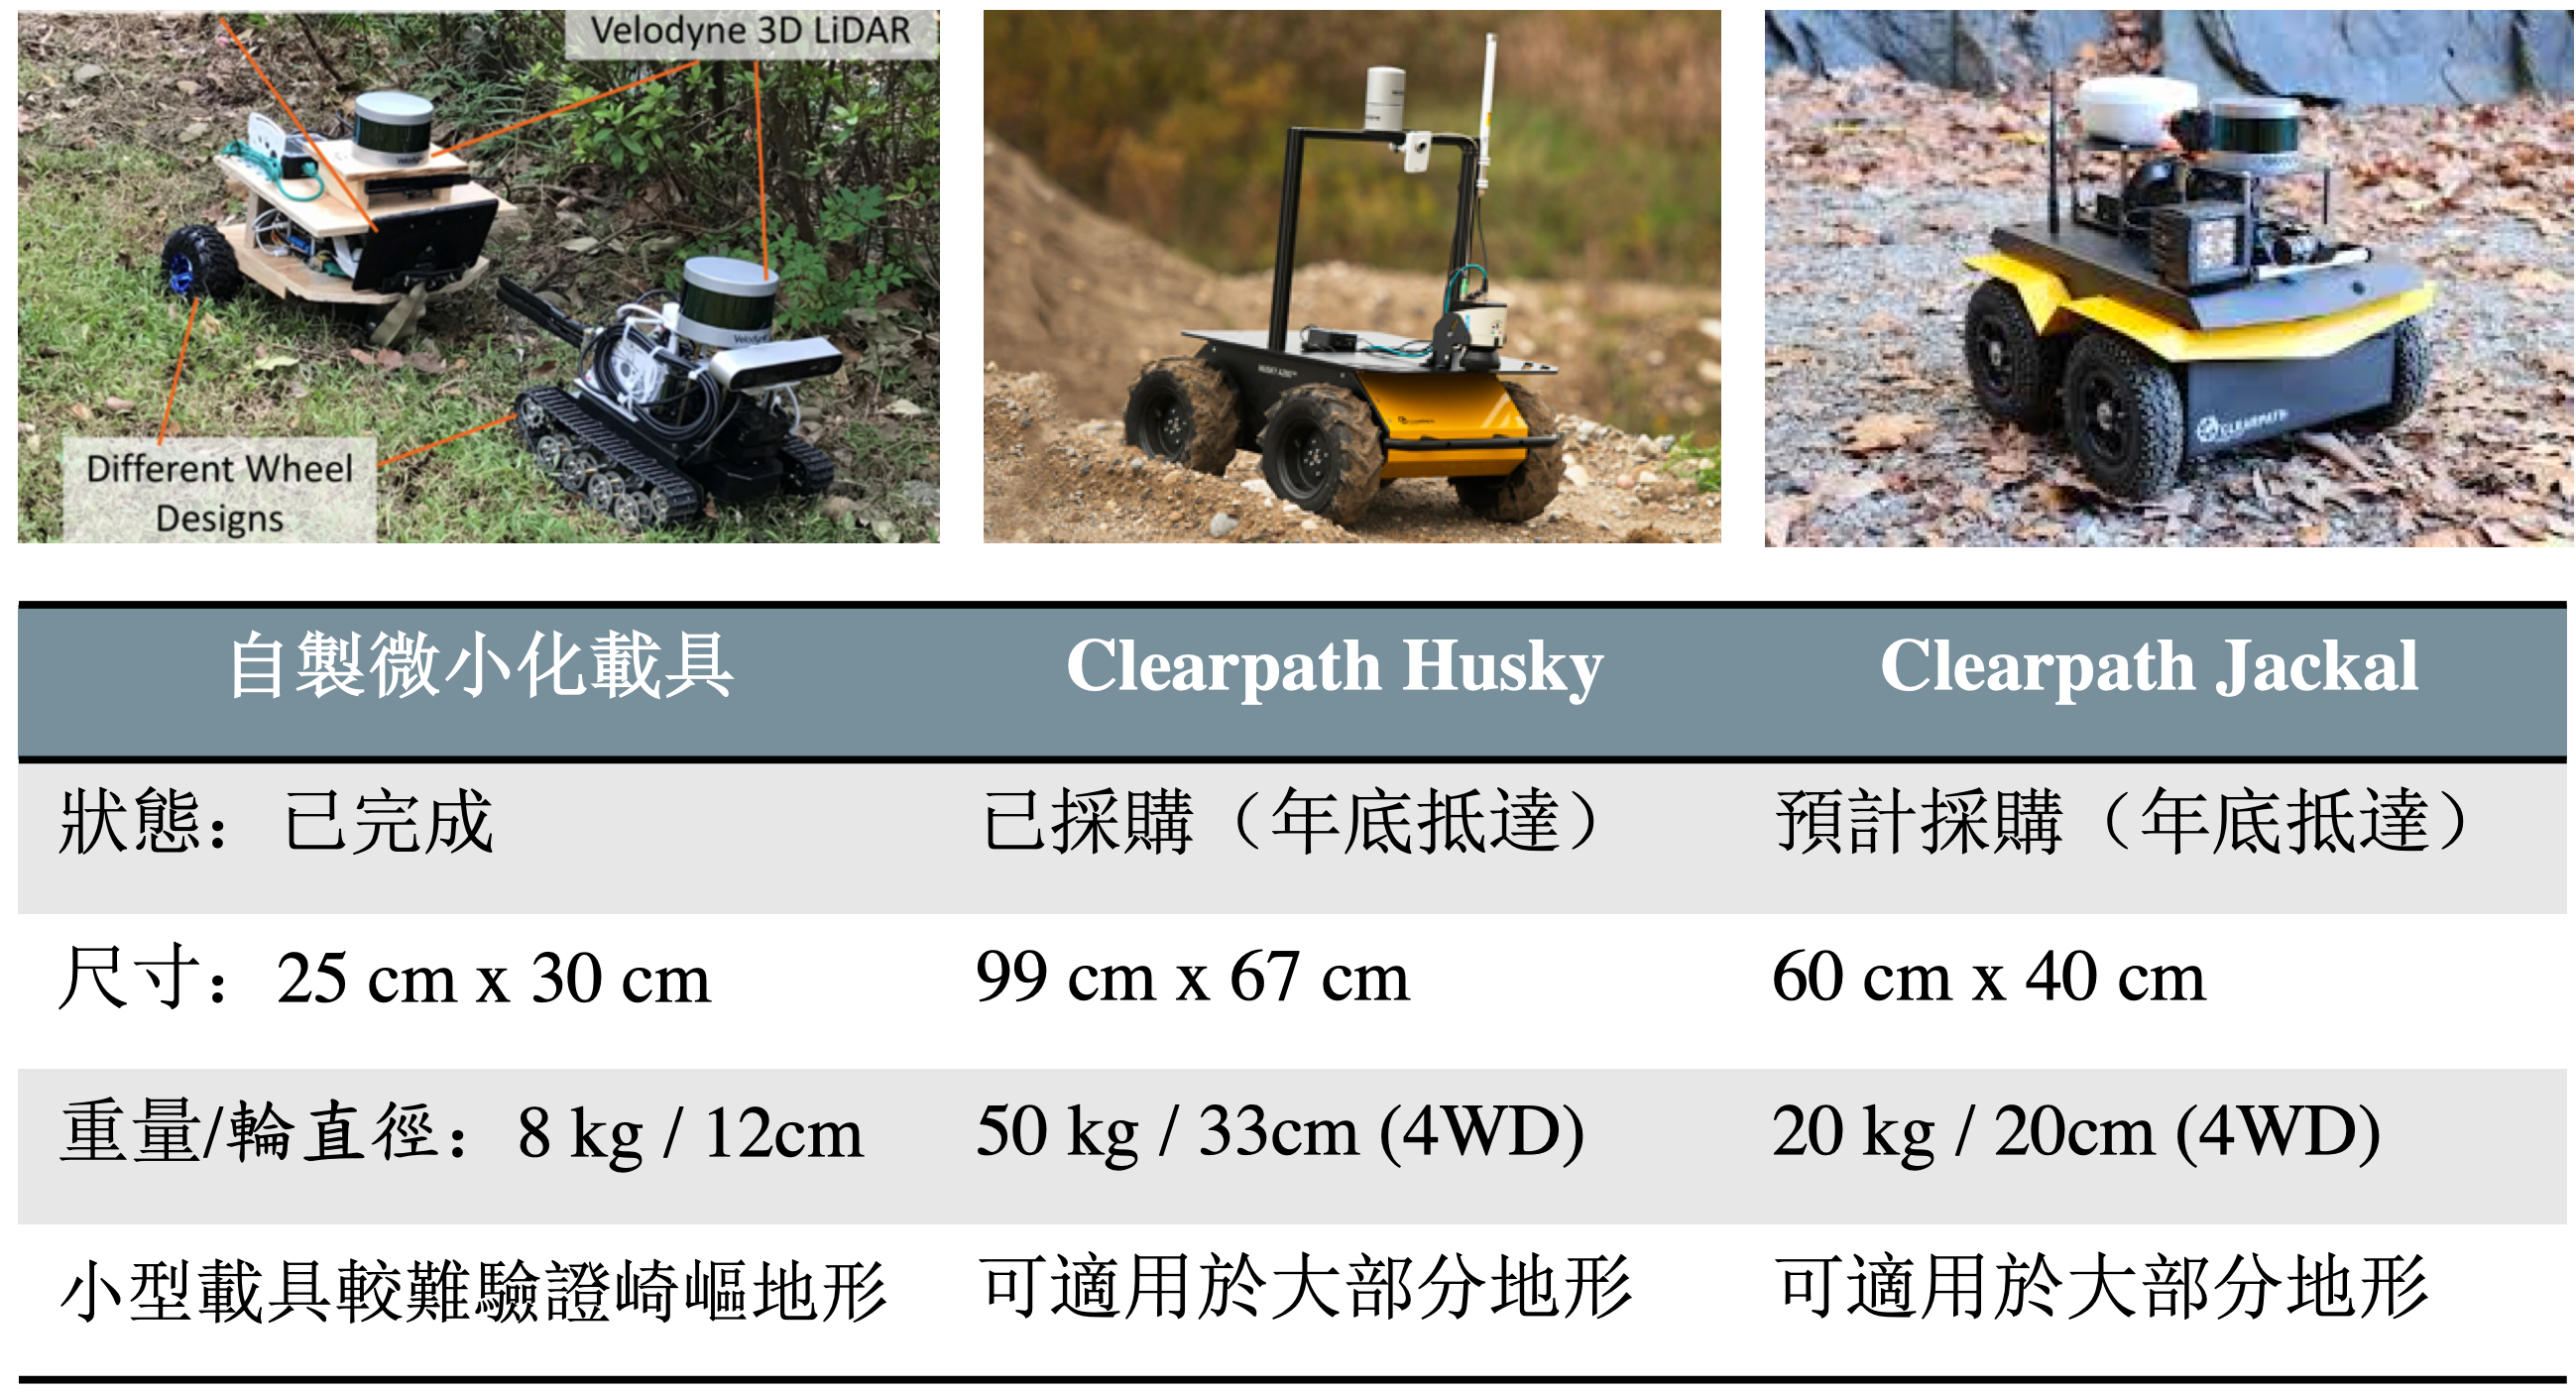
\includegraphics[width=\columnwidth]{images/ground-vehicle.png}
\centering
\caption{地面無人載具實際場域驗證}
 \label{figure:ground-vehicle}
\end{figure}

\subsection{水面無人載具與RobotX競賽(進行中)}

本計畫已將所開發之演算法用於大型水面無人載具,Marine Advanced Research 所提供的自適應性波浪快艇 (Wave Adaptive Modular Vessel, WAM-V),並透過設計此船隻的感測、計算、及動力完成競賽任務。本論文使用之自適應性波浪快艇系統架構圖如圖~\ref{figure:system_diagram}所示,其中主要分成三個部分: 硬體、電路、軟體,分別在模擬與實際竹湖場域測試。

\begin{figure}[bht]
	\centering
	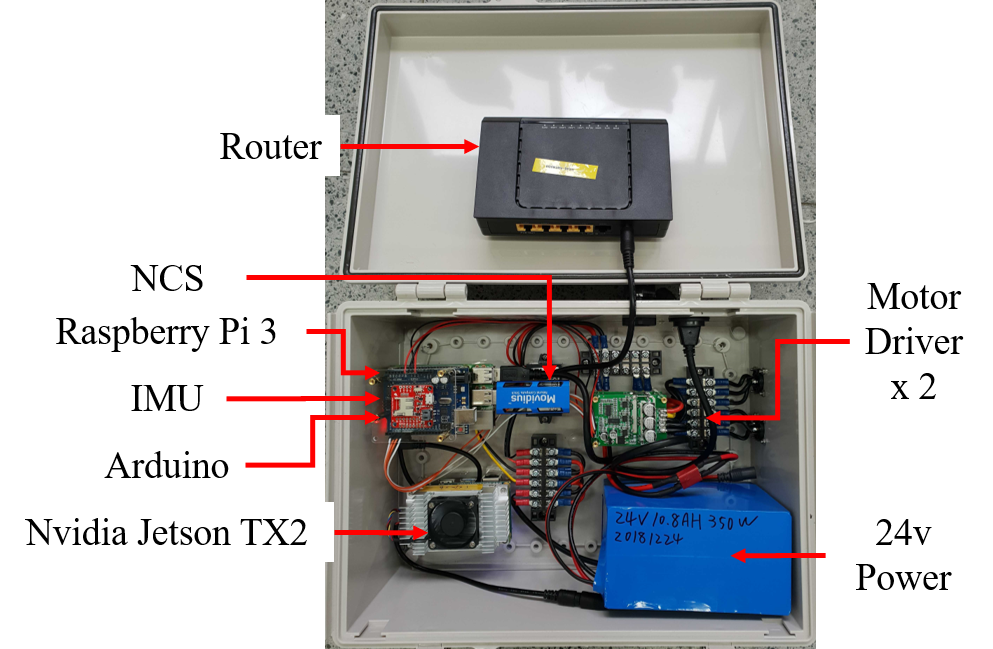
\includegraphics[height=!,width=\linewidth,keepaspectratio=true]
	{images/hardware_setting.png}
	\caption{本計畫將所開發的演算法移植到大型水上無人載具,將於2018年12月代表台灣第一次參與在夏威夷舉行的RobotX競賽。}
	\label{figure:system_diagram}
\end{figure}




    %\section{結論}

本計畫利用虛擬環境Gazebo開發測試無人載具演算法,建置多重感測器平台,並開發點雲資料融合建置崎嶇地形與障礙物模型,進而進行運動規劃與控制,已達成無人載具之定位、避障、導航等功能,本計畫將使用大型地面與水面無人載具,在實際場域進行測試。


    %\addtolength{\textheight}{-12cm} % This command serves to balance the column lengths
    % on the last page of the document manually. It shortens
    % the textheight of the last page by a suitable amount.
    % This command does not take effect until the next page
    % so it should come on the page before the last. Make
    % sure that you do not shorten the textheight too much.

    %%%%%%%%%%%%%%%%%%%%%%%%%%%%%%%%%%%%%%%%%%%%%%%%%%%%%%%%%%%%%%%%%%%%%%%%%%%%%%%%
    %\section*{APPENDIX}

    %Appendixes should appear before the acknowledgment.

    \section*{ACKNOWLEDGMENT}

    本研究感謝交大校長、副校長、機器人碩士學位學程、ICT工作坊、青年講座教授增能計畫、研發處學生出國競賽補助。台中中科管理局、工研院國際交流與國際競賽選手培訓計畫。
    Dr. Michael Benjamin, Prof. Henrik Schmidt (MIT)支持學生移地訓練。
    科技部國防科技計畫與中科院呂旺全先生於RobotX培訓課程機器人視覺演說,以及設備支持,最後感謝全體Team NCTU師生對本計畫的貢獻。

    %This work was partially
    %supported by the National Science Foundation under grants IIS-1318392 and
    %IIS-1405259.

    %%%%%%%%%%%%%%%%%%%%%%%%%%%%%%%%%%%%%%%%%%%%%%%%%%%%%%%%%%%%%%%%%%%%%%%%%%%%%%%%

    \bibliographystyle{IEEEtran}
    \bibliography{arg-egbib}

\end{CJK}
\end{document}